\chapter{Betriebsschwingungsanalyse}
\label{sec: Hauptkapitel 2}


\section{Aufgabenstellung}
%=========================
    % Grundziel
    %----------
    Ziel dieser Laboraufgabe ist das Durchführen einer Betriebsschwingungsanalyse
    mit anschließender Erstellung eines Campbell-Diagramms. Der Motor des
    Modellflugzeugs soll dabei von einem Elektromotor ohne Verdichtung
    geschleppt werden. Das Schwingungssignal soll an einem bestimmten Punkt der
    Tragfläche abgenommen werden.
%================================================================================

\section{Versuchsaufbau}
%=======================
    % Sensorplatzierung
    %------------------
    Obwohl nur ein Sensorsignal ausgewertet werden muss, werden 4
    Beschleunigungssensoren am vorderen Tragflügel positioniert platziert.
    Somit kann mit einem Aufbau und einer Messung sowohl die Aufgabe von Kapitel
    \ref{sec: Hauptkapitel 2} und Kaptiel \ref{sec: Hauptkapitel 3}
    abgewickelt werden. Die Beschleunigungssensoren werden an Punkten 1, 2, 4 und
    5 rot platziert (siehe Abbildung \ref{fig: Sensorpos_BSA}). Im Zuge von
    Kapitel \ref{sec: Hauptkapitel 2} wird der Messpunkt 5 rot verwendet und in
    weiterer Folge als Messpunkt 1 bezeichnet.

    % Bild - Sensorplatzierung BSA
    %-----------------------------
    \begin{figure}[H]
        \centering
        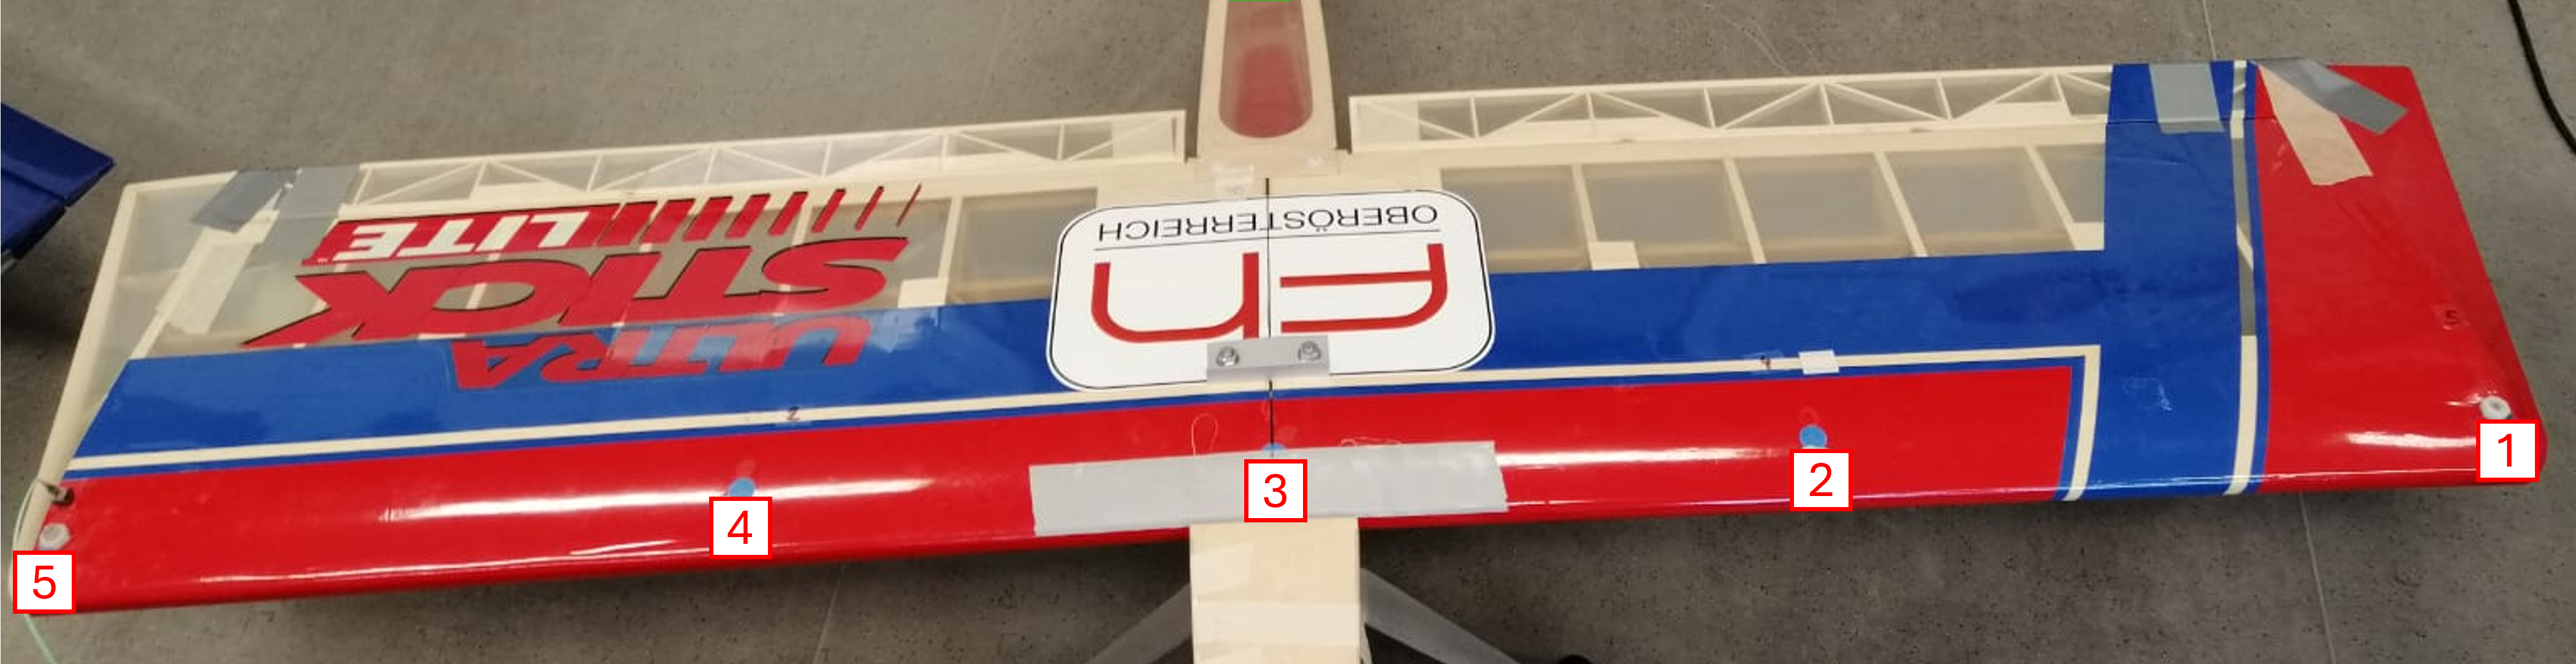
\includegraphics[width=0.9\textwidth]{BSA_Sensorpositionen.png}
        \caption{Sensorpositionen BSA}
        \label{fig: Sensorpos_BSA}
    \end{figure}
    %----------------------------------------------------------------------------

    % Fixierung Flieger
    %------------------
    \noindent
    Damit der Modellflieger bei den Messungen nicht durch die Schwingungen
    verfahren wird, wird er am Boden fixiert. Dazu werden behelfsmäßige Keile mit
    Klebeband am Boden bei den Rädern befestigt.
    \\
    %----------------------------------------------------------------------------

    % Messung mit Motor
    %------------------
    \noindent
    Bevor nun die Betriebsschwingungsanalyse durchgeführt werden kann, wird der
    Motor des Modellflugzeugs mit etwas Öl geschmiert. Dann wird der Elektromotor
    an die Welle zum Übertragen des Drehmoments angesetzt. Nun kann die Messung
    gestartet werden. Dabei wird der Elektromotor langsam mit einer Rampe von einer
    Spannung von 0 [V] auf 5 [V] beschleunigt. Während der Messung wird der
    Elektromotor in der Hand gehalten.
    %----------------------------------------------------------------------------

    % Drehzahlmessung
    %----------------
    \noindent
    Da das Ziel dieser Laboraufgabe die Erstellung eines Campbell-Diagramms ist,
    muss zusätzlich zum Beschleugingungssignal auch die Drehzahl des Motors
    aufgenommen werden. Dazu wird ein Beschleunigungssensor am Motorgehäuse
    angebracht und der Elektromotor mit einer konstanten Spannung betrieben. Da
    der Motor eine gewisse Unwucht aufweist, ist in regelmäßigen Abständen eine
    Spitze im Beschleugingungssignal zu sehen. Dadurch kann auf die Drehzahl
    rückgeschlossen werden. Anschließend wird eine 2. Messung mit einer höheren
    Spannung durchgeführt und erneut die Drehzahl bestimmt. Unter Annahme eines
    linearen Zusammenhangs zwischen Spannung und Drehzahl kann nun eine Funktion
    der Drehzahl in Abhängigkeit der Spannung gefunden werden. Die durchgeführten
    Messungen sind in Tabelle \ref{tab: Drehzahlmessung} zu sehen.
    %----------------------------------------------------------------------------

    % Tabelle - Drehzahlmessung
    %--------------------------
    \begin{table}[H]
        \centering
        \begin{tabular}{|c|c|c|}
            \hline
            \textbf{Spannung [V]} & \textbf{Frequenz [HZ]} & \textbf{Drehzahl [U/min]} \\
            \hline \hline
            1   &   8   &   480 \\
            \hline
            2   &   17.5    &   1050 \\
            \hline
            4   &   36.6    &   2196 \\
            \hline
        \end{tabular}
        \caption{Messungen zur Bestimmung der Drehzahl}
        \label{tab: Drehzahlmessung}
    \end{table}
    %----------------------------------------------------------------------------

    % Erklärung - Centerpoint
    %------------------------
    \noindent
    Wie in Tabelle \ref{tab: Drehzahlmessung} zu sehen ist, wurde auch eine 3.
    Messung durchgeführt. Diese dient als Centerpoint-Messung und soll
    überprüfen, ob auch wirklich ein linearer Zusammenhang vorliegt. In Abbildung
    \ref{fig: Drehzahlmessung} sind die 3 Messungen in einem Diagramm dargestellt.

    % Bild - Drehzahlmessung
    %-----------------------
    \begin{figure}[H]
        \centering
        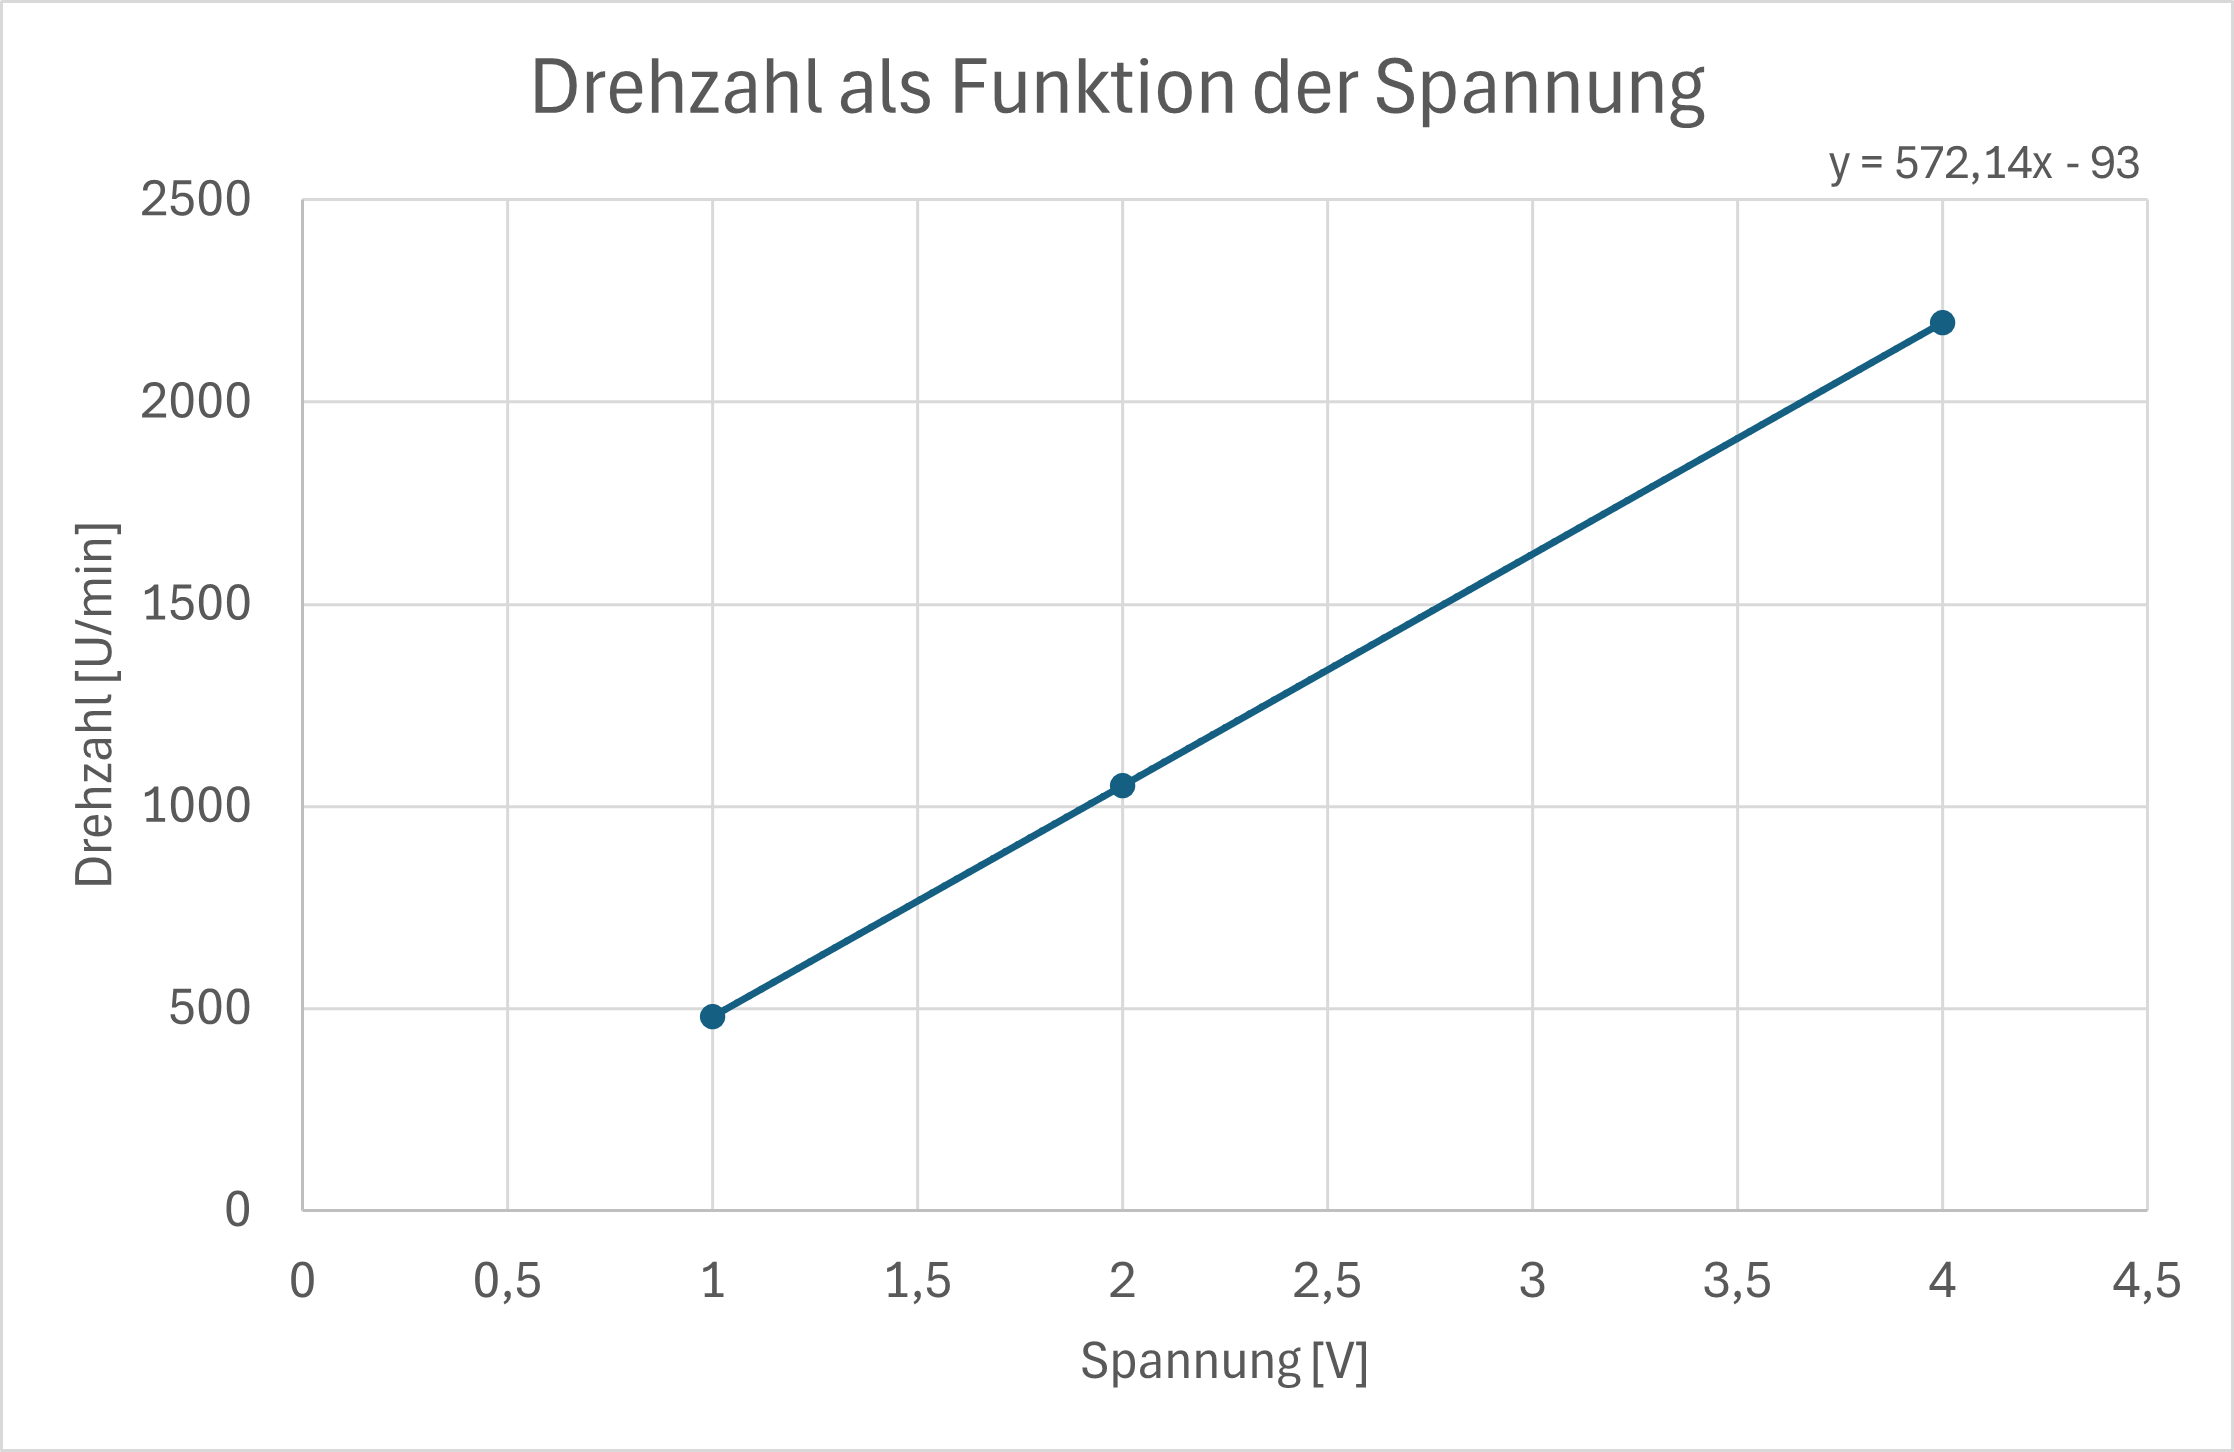
\includegraphics[width=0.7\textwidth]{Drehzahlmessung.png}
        \caption{Zusammenhang zwischen Spannung und Drehzahl}
        \label{fig: Drehzahlmessung}
    \end{figure}


%================================================================================

\section{Ergebnisse}


